\documentclass[a4paper, titlepage]{jsarticle}

\usepackage[dvipdfmx]{graphicx}
\usepackage{amsmath}
\usepackage{mathtools}
\usepackage{listings}

\lstset{
  basicstyle={\ttfamily},
  identifierstyle={\small},
  commentstyle={\smallitshape},
  keywordstyle={\small\bfseries},
  ndkeywordstyle={\small},
  stringstyle={\small\ttfamily},
  frame={tb},
  breaklines=true,
  columns=[l]{fullflexible},
  numbers=left,
  xrightmargin=0zw,
  xleftmargin=3zw,
  numberstyle={\scriptsize},
  stepnumber=1,
  numbersep=1zw,
  lineskip=-0.5ex
}

\title{シミュレーション工学Ⅱ モンテカルロ法}
\author{三浦夢生}
\date{2020.11.11 Wed}

\begin{document}
	\maketitle

	\section{モンテカルロ法}
	モンテカルロ法とは数値計算分野において乱数を用いて行う手法の総称であるが,今回は乱数を用いて面積の近似解を求める方法のことを指して使う.
	乱数を用いるため,品質の良い疑似乱数生成アルゴリズムを選ぶ必要がある.

	ある領域の面積$S$を求めたい場合,その領域を含む面積$T$の中にランダムに点を打ち,領域内に点が含まれる確率$p$を用いて$S=pT$と書ける.

	有名なものでは,モンテカルロ法を用いて円周率を求めるものがある.

	\section{乱数生成器}
	\subsection{線形合同法}
	疑似乱数を生成する方法の一つで,以下の式で示される.
		\begin{equation}
			X_{n+1}=(A*{X_n}+B)\bmod{M}
		\end{equation}
	ここで$X_0$は初期値(シード値),$A,B,M$はパラメータであり,この値のとり方によって疑似乱数の質が変わる.この方法は一般にあまり質が良くないとされる.

	\subsection{メルセンヌ・ツイスタ}
	高次元に均等分布する乱数を高速に生成できる非常に評価の高い疑似乱数生成器である.内部状態の大きさや周期は設定可能であるが,基本的に$2^{19937}-1$が用いられる.他の疑似乱数生成器がもつ多くの欠点を克服しているため広く利用されている.

	\section{円周率}
	\subsection{ライプニッツの公式}
	円周率を求めるための公式の一つで,以下の級数で示される.
		\begin{equation}
			1-\frac{1}{3}+\frac{1}{5}-\frac{1}{7}+\frac{1}{9}-\cdots=\frac{\pi}{4}
		\end{equation}
	総和の記号を用いると以下のようにも表せる.
		\begin{equation}
			\sum_{n=0}^{\infty}\frac{(-1)^n}{2n+1}=\frac{\pi}{4}
		\end{equation}
	美しくまとまっているが,収束が遅いことで知られる.

	\subsection{マチンの公式}
	マチンは$\arctan{x}$の関係式を考え,グレゴリー級数と結びつけてより速く収束する級数を得た.それを以下に示す.
		\begin{equation}
			4\arctan\frac{1}{5}-\arctan\frac{1}{239}=\frac{\pi}{4}
		\end{equation}
	計算においては上記の公式の両辺を4倍し,$\arctan{x}$をグレゴリー級数に直して差を取る.
		\begin{equation}
			d(m)=16\sum_{n=0}^{3m+2}\frac{(-1)^n}{2n+1}\left(\frac{1}{5}\right)^{2n+1}-4\sum_{n=0}^{m}\frac{(-1)^4}{2n+1}\left(\frac{1}{239}\right)^{2n+1}
		\end{equation}
	ここで,第1項と第2項の項数が違うのは,$\frac{1}{5}$と$\frac{1}{239}$で値が大きく異なるため,項全体の値の大きさを近づけるためである.
	
	\subsection{ラマヌジャンによる公式}
	ラマヌジャンはモジュラー関数と呼ばれる考えをもとに以下の式を発見した.
		\begin{equation}
			\frac{1}{\pi}=\frac{2\sqrt{2}}{99^2}\sum_{n=0}^{\infty}\frac{(4n)!(1103+26390n)}{(4^{n}99^{n}n!)^4}
		\end{equation}
	この公式は非常に収束が速いことで知られる.

	\section{課題}
	\subsection{課題1}
	積分2問の手計算した画像を以下に示す.
		\begin{figure}[ht]
			\centering
			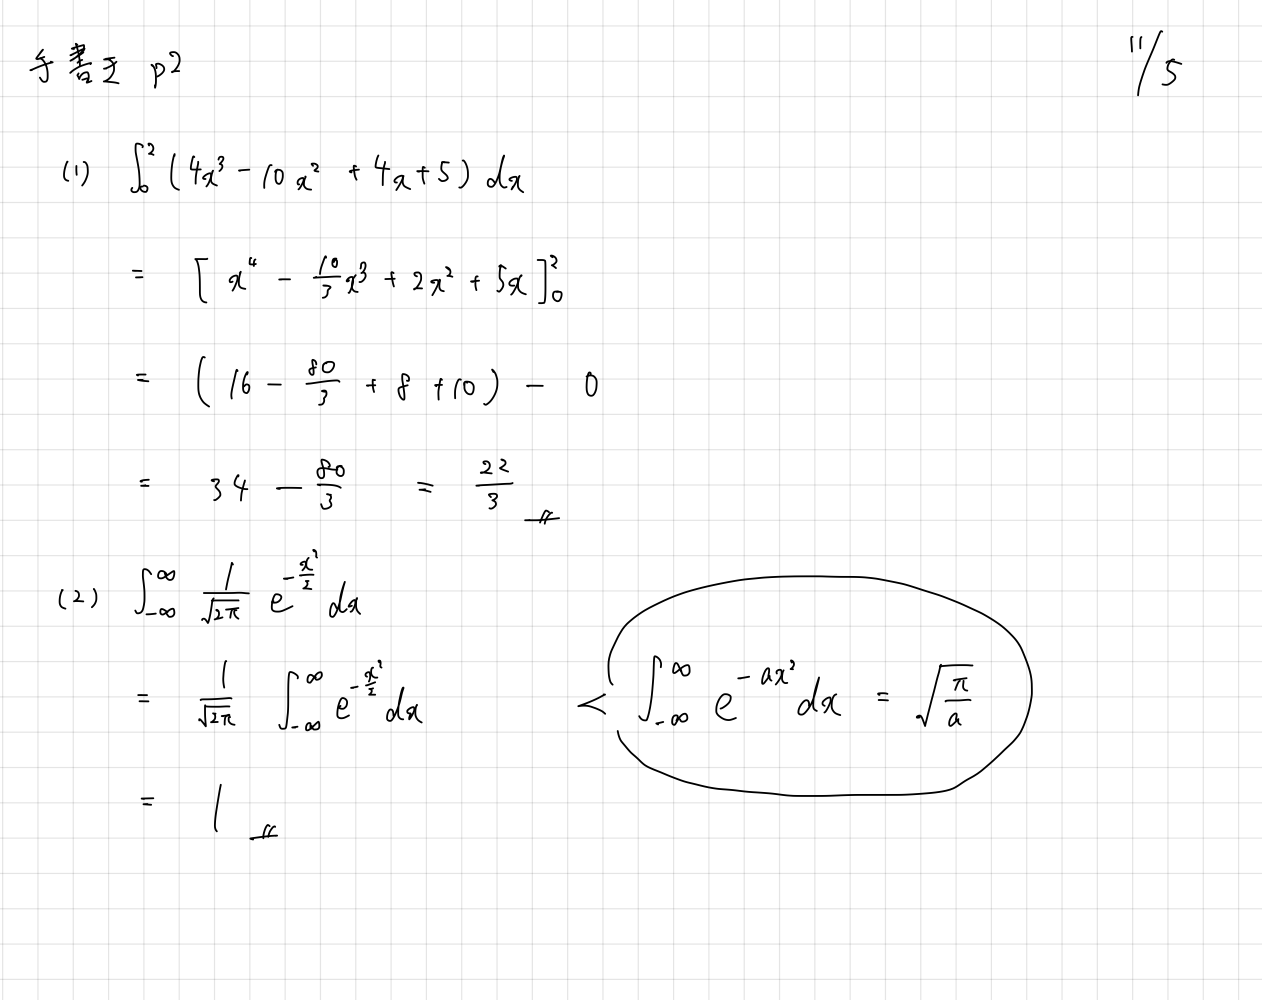
\includegraphics[keepaspectratio, scale=0.2]{File_001.png}
		\end{figure}

	\subsection{課題2}
	上記と同様の問題をモンテカルロ法のプログラムで解いた結果を以下に示す.ただし,問2の積分範囲は$-5 {\leq} x {\leq} 5$としている.
	またプログラムリストを付録に示す.
		\begin{lstlisting}
% python3 MonteCarlo1.py
S = 7.33278
		\end{lstlisting}
		\begin{lstlisting}
% python3 MonteCarlo2.py
S = 0.9974
		\end{lstlisting}

	\subsection{課題3}
	自作の線形合同法とメルセンヌ・ツイスタで乱数を生成し,円周率を求めた結果を以下に示す.
	またプログラムリストを付録に示す.
		\begin{lstlisting}
% python3 pi2_1.py
pi = 3.14872
		\end{lstlisting}
		\begin{lstlisting}
% ./MT_pi
pi = 3.147680
		\end{lstlisting}
	後述のプログラムリストの通り,ランダムデータの数が少ないためあまり比較が出来なかった.

	\subsection{課題4}
	先述した3つの方法で円周率を求めた結果を以下に示す.
	またプログラムリストを付録に示す.
		\begin{lstlisting}
% python3 pi1.py
n = 1000000
leibniz: 3.1415936535887745
n = 10
machin: 3.141592653589794
n = 1
ramanujan: 3.141592653589794
		\end{lstlisting}
	試行回数からわかるように収束の速さに違いが見られる.

	\section{付録}
	今回作成したプログラムを以下に示す.

	\subsection{モンテカルロ法積分プログラム1}
		\begin{lstlisting}
import numpy as np

def func(x):
   return 4*(x**3) - 10*(x**2) + 4*x + 5

def generate_random(a, b, maxY, t):
    dataX = []
    dataY = []
    dataX = np.random.rand(t) * (b - a) + a
    dataY = np.random.rand(t) * maxY
    return dataX, dataY

def montecarlo(t, dataX, dataY):
    cnt = 0
    for i in range(len(dataX)):
        if func(dataX[i]) >= dataY[i]:
            cnt += 1
    p = float(cnt) / float(t)
    return p

if __name__ == '__main__':
    t = 1000000
    a = 0
    b = 2
    maxY = 10
    cnt = 0

    dataX, dataY = generate_random(a, b, maxY, t)
    p = montecarlo(t, dataX, dataY)
    print('S =', (b-a) * maxY * p)
		\end{lstlisting}

	\subsection{モンテカルロ法積分プログラム2}
		\begin{lstlisting}
import numpy as np

def func(x):
		return (1/np.sqrt(2*np.pi)) * np.exp(-(x**2)/2)

def generate_random(a, b, maxY, t):
    dataX = []
    dataY = []
    dataX = np.random.rand(t) * (b - a) + a
    dataY = np.random.rand(t) * maxY
    return dataX, dataY

def montecarlo(t, dataX, dataY):
    cnt = 0
    for i in range(len(dataX)):
        if func(dataX[i]) >= dataY[i]:
            cnt += 1
    p = float(cnt) / float(t)
    return p

if __name__ == '__main__':
    t = 1000000
    a = -5
    b = 5
    maxY = 2
    cnt = 0

    dataX, dataY = generate_random(a, b, maxY, t)
    p = montecarlo(t, dataX, dataY)
    print('S =', (b-a) * maxY * p)
		\end{lstlisting}

	\subsection{線形合同法円周率プログラム}
		\begin{lstlisting}
def generate_point(times):
    dataX = LCGs(times, 1)
    dataX = [i / 2**32 for i in dataX]
    dataY = LCGs(times, 2)
    dataY = [i / 2**32 for i in dataY]
    return dataX, dataY

def LCGs(num, seed):
    A = 1664525
    C = 1103515245
    M = 2**32
    x = seed
    r_list = []
    for i in range(num):
        x = (A * x + C) % M
        r_list.append(x)
    return r_list

def count_point(dataX, dataY):
    cnt = 0
    for x, y in zip(dataX, dataY):
        if x**2 + y**2 < 1:
            cnt += 1
    return cnt

def main():
    times = 100000

    dataX, dataY = generate_point(times)
    cnt = count_point(dataX, dataY)
    print('pi =', 4 * cnt / times)

if __name__ == '__main__':
    main()
		\end{lstlisting}

	\subsection{メルセンヌ・ツイスタ円周率プログラム}
		\begin{lstlisting}
#include <stdio.h>
#include "MT.h"

#define NUM 100000

int count_point(double dataX[NUM], double dataY[NUM]);

int main(void)
{
	int i;
	int seed;
	int cnt;
	double pi;
	double dataX[NUM];
	double dataY[NUM];

	seed = 0;
	init_genrand(seed);

	for (i = 0; i < NUM; i++) {
		dataX[i] = genrand_real1();
		dataY[i] = genrand_real1();
	}

	cnt = count_point(dataX, dataY);
	pi = 4 * (double)cnt / (double)NUM;

	printf("pi = %lf\n", pi);

	return 0;
}

int count_point(double dataX[NUM], double dataY[NUM])
{
	int i;
	int cnt;

	cnt = 0;

	for (i = 0; i < NUM; i++) {
		if (dataX[i] * dataX[i] + dataY[i] * dataY[i] < 1) {
			cnt++;
		}
	}

	return cnt;
}
		\end{lstlisting}

	\subsection{ライプニッツ・マチン・ラマヌジャン円周率プログラム}
		\begin{lstlisting}
import math

def leibniz():
    n = 1000000
    print('n =', n)
    s = 0.0
    for i in range(n+1):
        s += (-1)**i / ((2*i) + 1)
    pi = s * 4
    return pi

def machin():
    n = 10
    print('n =', n)
    num_1 = 0.0
    for i in range(3*n+2+1):
        num_1 += ((-1)**i / (2*i+1)) * ((1/5)**(2*i+1))
    num_1 = num_1 * 16
    num_2 = 0.0
    for i in range(n+1):
        num_2 += ((-1)**i / (2*i+1)) * ((1/239)**(2*i+1))
    num_2 = num_2 * 4
    pi = num_1 - num_2
    return pi

def ramanujan():
    n = 1
    print('n =', n)
    s = 0.0
    for i in range(n+1):
        temp1 = 1
        for j in reversed(range(1, 4*i+1)):
            temp1 *= j
        temp2 = 1
        for j in reversed(range(1, i+1)):
            temp2 *= j
        s += (temp1 * (1103+26390*i)) / (((4**i) * (99**i) * temp2))**4
    s = s * 2 * math.sqrt(2) / (99**2)
    pi = 1 / s
    return pi

if __name__ == '__main__':
    pi_1 = leibniz()
    print('leibniz:', pi_1)
    pi_2 = machin()
    print('machin:', pi_2)
    pi_3 = ramanujan()
    print('ramanujan:', pi_3)
		\end{lstlisting}

\end{document}
